\section{Historical protocol and implementation}
\subsection{Dataset, feature availability, and chronological partitions}
The source network archive contains 22,339,021 rows. The preprocessing manifest records 869 invalid rows and 22,338,152 retained rows. The retained input vector contains eight numerical fields in this order: \code{duration}, \code{src_bytes}, \code{dst_bytes}, \code{missed_bytes}, \code{src_pkts}, \code{src_ip_bytes}, \code{dst_pkts}, and \code{dst_ip_bytes}. Binary labels distinguish normal traffic from attacks. The eight-feature contract was inherited from the project's compact-detector experiments: it uses flow-level numerical aggregates without IP identifiers, ports, application strings, or categorical encodings. Holding it fixed makes the adaptation intervention comparable, but is not a feature-optimality claim. The chronological evaluation stream retains its observed prevalence.

Records are ordered by their complete-feature availability time,
\begin{equation}
 t_{\mathrm{ready}}=t_{\mathrm{start}}+\mathrm{duration}.
 \label{eq:ready}
\end{equation}
This is an offline flow-completion replay. It does not assume that duration or byte totals are known at the first packet. The retained data cover ten UTC calendar days in April 2019, with no retained interval from 5 to 22 April. Table~\ref{tab:data} defines the four chronological partitions. A estimates the initial transformation and model; B selects the initial threshold; C supports development; and D is reserved for the final predictive campaign.

\begin{table}[tb]
\centering\small
\caption{Chronological data partitions. Counts refer to retained rows; normal and attack counts sum to each partition total. The separate overlap strata are described in Section~\ref{sec:overlap}.}
\label{tab:data}
\begin{tabular}{llrrr}
\toprule
Partition & UTC dates, April 2019 & Total & Normal & Attack \\
\midrule
A: initial fit & 2--4, 23 & 3,956,308 & 223,199 & 3,733,109 \\
B: initial threshold & 24 & 5,681,198 & 89,323 & 5,591,875 \\
C: development & 25--26 & 9,150,673 & 173,316 & 8,977,357 \\
D: final evaluation & 27--29 & 3,549,973 & 309,673 & 3,240,300 \\
\bottomrule
\end{tabular}
\end{table}

Attack composition changes across these intervals. A contains scanning attacks; B contains scanning and denial of service. C contains distributed denial of service, denial of service, injection, and password attacks. D contains backdoor, man-in-the-middle, password, ransomware, and cross-site scripting records. These changes provide temporal heterogeneity, but the experiment does not identify a causal type of drift. Backdoor, man-in-the-middle, ransomware, and cross-site scripting are absent from A/B/C; password also occurs in C. The extension reports per-family attack recall.

Before the final campaign, D had been read for structural checks and feature-vector overlap analysis. Its predictive evaluation was run only after the protocol and code were fixed. Accordingly, D is a later evaluation interval, not a completely unseen resource in the broader research process. The five initial models and their B thresholds are prepared before the final runner loads D. C is used in that runner to construct the prior-vector inventory; the C adaptive state is not carried into D.

\subsection{Initial model and restricted adaptation}
Each raw input is transformed by $\log(1+\max(x,0))$ and standardized using means and standard deviations estimated from A. A zero standard deviation is replaced by one. The transformation remains fixed. Each transformed feature is then mapped to its range observed in A and clipped to $[0,1-10^{-9}]$ for spline evaluation. Values outside the observed range therefore saturate at a boundary rather than extrapolating the spline.

For input $j$, the model contains eight cubic B-spline basis functions $B_{jr}$ with an open knot vector based on six equally spaced positions between zero and one. The initial function is
\begin{equation}
 f_j(x_j)=\sum_{r=1}^{8}\theta_{jr}B_{jr}(u_j(x_j)),
 \qquad s(x;g,b)=b+\sum_{j=1}^{8}g_j f_j(x_j).
 \label{eq:model}
\end{equation}
The 64 spline coefficients and initial intercept are fitted by logistic regression on a uniform, seeded 400,000-row sample of A. The implementation uses scikit-learn with \code{C=1.0} and \code{max_iter=1000} \citep{pedregosa2011}. The initial gains are $g_j=1$. Subsequent adaptation leaves the transformation, knots, and all $\theta_{jr}$ fixed, and refits only the eight gains and intercept on the current fitting memory. Each refit solves a new logistic-regression problem with L2 shrinkage of the eight weights toward zero and an unpenalized intercept. It neither starts from nor penalizes distance to the previous head. The fixed spline functions retain information from A, while the head is newly fitted to the current memory. The extension explicitly tests a penalty centred at the previous head.

The empirical object is a logistic generalized additive model with an adaptive linear combination of fixed spline functions. Head refitting can reweight these functions, but cannot learn a new spline shape or an interaction between inputs.

\subsection{Threshold objective and four paired traces}
The implementation predicts attack when $s(x)>\tau$ and normal otherwise. For labeled set $\mathcal{L}$, the threshold objective is
\begin{equation}
 \tau^{*}(\mathcal{L},s)\in\arg\max_{\tau\in\mathcal{T}}
 \frac{1}{2}\left[\frac{\mathrm{TP}(\tau)}{P}+
 \frac{\mathrm{TN}(\tau)}{N}\right],
 \label{eq:threshold}
\end{equation}
where $P$ and $N$ are the attack and normal counts in $\mathcal{L}$. Candidates comprise the distinct observed scores and a floating-point value strictly below the minimum; together with the maximum observed score, this covers the all-attack and all-normal decisions. Scores and objective values use float64. Maximizers are selected by exact equality, without a tolerance, and ties are resolved by the lower median of the sorted maximizing candidates, at zero-based index $\lfloor(m-1)/2\rfloor$. This is a deterministic convention, not a demonstrated threshold-stability property.

The B threshold is selected separately for each initial model using all of B, then kept fixed in the corresponding B traces. Table~\ref{tab:traces} defines the four traces. Both frozen traces use identical initial scores; both FIT192 traces use an identical adapted score trajectory. Consequently, a threshold-only contrast cannot change AUROC. All traces share the same label requests and update eligibility decisions within a seed.

\begin{table}[tb]
\centering\small
\caption{Four paired traces. B denotes the initial fixed threshold; ROLE64 denotes recent threshold selection. The primary contrast is the last row minus the second row.}
\label{tab:traces}
\begin{tabularx}{\linewidth}{lXX}
\toprule
Trace & Score function & Decision threshold \\
\midrule
Frozen / B & Initial A model & Fixed, selected on B \\
Frozen / ROLE64 & Initial A model & Selected on recent ROLE64 labels \\
FIT192 / B & Head refitted on FIT192 & Fixed, selected on B \\
FIT192 / ROLE64 & Same refitted head as FIT192 / B & Selected on recent ROLE64 labels \\
\bottomrule
\end{tabularx}
\end{table}

\subsection{Label budget, delay, and memory separation}
D is divided into 354 blocks of 10,000 records and a final block of 9,973 records, indexed from 0 to 354. Predictions for a block are emitted before any labels from that block enter the controller. A uniform sample without replacement requests $\lfloor0.01 n_k\rfloor$ labels from block $k$: 100 from a full block and 99 from the last block. Requested labels arrive at the end of block $k+1$ and can first influence predictions in block $k+2$ (Figure~\ref{fig:protocol}). Thus 35,499 labels are requested, of which the final 99 remain pending when the observed stream ends. Full labels are available only to the offline evaluation code; the online update receives the delayed requested subset.

\begin{figure}[tb]
\centering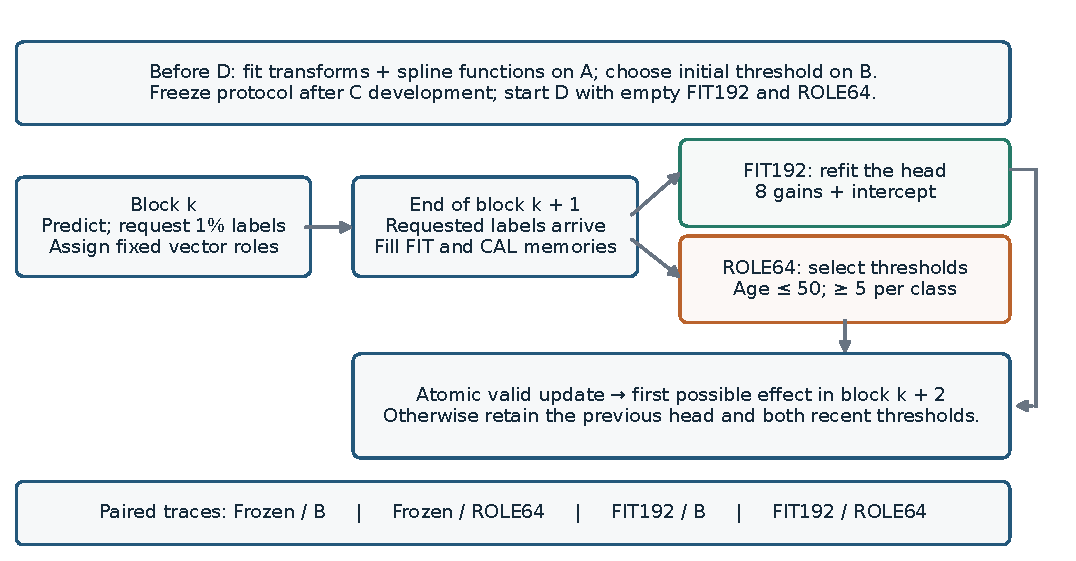
\includegraphics[width=\linewidth]{figures/fig1_protocol.pdf}
\caption{Causal protocol. A label requested in block $k$ cannot affect predictions before block $k+2$. Fitting and threshold selection use separate memories; all state changes are committed together only after the eligibility checks succeed.}
\label{fig:protocol}
\Description{Causal protocol. A label requested in block $k$ cannot affect predictions before block $k+2$. Fitting and threshold selection use separate memories; all state changes are committed together only after the eligibility checks succeed.}
\end{figure}

Both memories start empty at the beginning of D. FIT192 holds at most 192 labeled examples, with target quotas of 96 normal and 96 attack examples. ROLE64 holds at most 64 examples, with target quotas of 32 per class. Either class can borrow unused capacity. On overflow, the oldest example from a class above quota is removed. The quotas alter the stored fitting and threshold-selection samples, not the evaluation stream or the requested-label budget.

A fixed salted SHA-256 rule assigns each raw eight-feature vector permanently to one role: digest modulo four equal to zero selects CAL, and other values select FIT. This prevents an identical vector from appearing in both fitting and calibration memories, even if it recurs later in the stream. It does not deduplicate either memory internally. Role serialization uses canonical float64 bytes; exact overlap between chronological partitions is measured separately using the stored float32 vectors. Appendix~\ref{sec:implementation} specifies these encodings.

FIT192 requires both binary classes. ROLE64 contributes only entries observed at most 50 blocks earlier and requires at least five normal and five attack labels. FIT192 has no corresponding age cutoff. If these conditions hold, the implementation fits a candidate head, scores the eligible ROLE64 examples with both the frozen and candidate heads, and computes two thresholds using Equation~\ref{eq:threshold}. A valid candidate head and both thresholds replace the prior state atomically for the next block. A failed eligibility or numerical check leaves all prior state unchanged and records the reason.

This common schedule isolates the effect of enabling head fitting within the fixed controller, while keeping threshold data and update eligibility matched. It does not estimate a benefit per additional label: FIT192/ROLE64 can use FIT-role labels that Frozen/ROLE64 leaves unused. The extension therefore adds independently eligible ROLE64 and a frozen ALL256 control that can use every acquired label. The 256-example capacity also excludes the delayed-label queue, model state, feature transformations, Python object overhead, temporary solver arrays, and full input arrays used by the offline runner. It must not be interpreted as a total memory bound for an embedded implementation.

\subsection{Overlap-aware reporting}\label{sec:overlap}
The chronological partitions have disjoint row identities, but their eight-feature vectors overlap. An exact SHA-256 inventory of A/B/C marks each D vector as previously observed or unobserved. In D, 37.23\% of rows and 58.03\% of normal rows match a prior vector. The unobserved-vector mask retains 2,228,436 rows: 129,982 normal and 2,098,454 attack observations. The complementary seen stratum contains 179,691 normal and 1,141,846 attack observations.

This mask is applied only when aggregating predictions. It changes neither the prediction sequence nor the adaptive state. Requested labels from all of D can still enter the controller, and repetitions within D remain. The supplementary result therefore measures performance on vectors absent from A/B/C during the same adaptive replay. It is not a separately trained no-overlap experiment, an unseen-attack-family test, or a guarantee that a vector has never previously affected the state within D. A matching eight-feature vector is also not proof that two original network events are duplicates.

\subsection{Metrics, paired seeds, and decision criterion}
We report global false negatives (FN), false positives (FP), attack recall $\mathrm{TP}/P$, false-positive rate $\mathrm{FP}/N$, and balanced accuracy
\begin{equation}
 \mathrm{BA}=\tfrac12\left(\mathrm{recall}+1-\mathrm{FPR}\right).
\end{equation}
These rates are computed from the confusion matrix aggregated over the selected scope. Ranking is summarized by the unweighted mean of AUROC over blocks containing both classes:
\begin{equation}
 \meanauc=\frac{1}{|\mathcal{V}|}\sum_{k\in\mathcal{V}}\mathrm{AUC}_k.
\end{equation}
Undefined AUROCs remain missing. Valid denominators are 352 of 355 blocks for all D and 350 of 355 for the A/B/C-unseen subset. This statistic is not the AUROC obtained by pooling every score across the stream; it does not require scores from different adaptive states to be directly comparable.

Seeds 42--46 determine the initial A subsample and block-level label sampling. The original sampler initializes each block with seed+k; different seed/block pairs can therefore reuse the same relative query positions. The extension replaces this with a tuple-keyed SeedSequence while retaining common requests across methods. Each seed shares all observations and requests across its four traces. Values are means and sample standard deviations ($n-1$ denominator) over the five seeds. Differences are computed within seed before aggregation. These deviations describe stochastic variation conditional on one recorded stream; they are neither confidence intervals nor variation across five independent datasets.

The versioned protocol fixed the primary comparison as FIT192 / ROLE64 minus Frozen / ROLE64. Its decision criterion required $\Delta\mathrm{FN}\leq0$ and $\Delta\mathrm{FP}\leq0$, with at least one strict inequality, in at least four of five seeds. This is a pre-specified empirical acceptance rule, not a statistical significance test or an externally registered trial. The full-stream and supplementary outcomes are reported whether or not the criterion succeeds. We do not select a new operating threshold using final D outcomes.

